
\begin{document}

\section{Balanced Scorecard}
\item{El Balanced Scorecard (BSC) o Cuadro de Mando Integral (CMI) es una herramienta de gestión que permite implementar la estrategia de una empresa a partir de una serie de medidas de actuación, permitiendo un control permanente sobre todos los factores de la organización, interrelacionando objetivos y relacionándolos con acciones concretas.}

\begin{center}
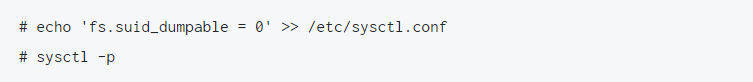
\includegraphics[width=15cm]{./Imagenes/imagen1}
\end{center}

\section{¿Cómo funciona el Balanced Scorecard?}
\item{El proceso de creación de un BSC comienza con la determinación de los siguientes parámetros:\\\\
-Objetivos a alcanzar por la organización.\\
-Indicadores o mediciones más adecuados para poder controlar el grado de alance de los objetivos.\\
-Metas concretas en relación a los resultados específicos de dichas mediciones.\\
-Acciones, iniciativas proyectos o programas que se van a implementar para lograr dichas acciones.\\\\
Una vez fijados todos estos factores, el siguiente paso es colocar todas estas mediciones, metas y objetivos en un panel o cuadro, utilizando para ellos un software específico donde se monitorea el progreso de cada uno de ellos.\\
Los datos, que normalmente se obtienen de los sistemas informáticos de la empresa, se presentan de manera esquemática y muy gráfica en un panel similar al que utilizan los pilotos de aviones, por lo que también se le conoce como «Cuadro de Mando Integral».}

\section{Perspectivas del Balanced Scorecard}
\item{A pesar de que son 4 las perspectivas que tradicionalmente identifican un BSC, no es indispensable que estén todas ellas; estas perspectivas son las más comunes y pueden adaptarse a la gran mayoría de las empresas, y no constituyen una condición indispensable para construir un modelo de negocios.\\\\\
\textbf{Perspectiva financiera}\\
Históricamente los indicadores financieros han sido los más utilizados, pues son el reflejo de lo que está ocurriendo con las inversiones y el valor añadido económico, de hecho, todas las medidas que forman parte de la relación causa-efecto, culminan en la mejor actuación financiera.Información administrada por un sistema ERP.\\\\
\textbf{Perspectiva del cliente}
Como parte de un modelo de negocios, se identifica el mercado y el cliente hacia el cual se dirige el servicio o producto. La perspectiva del cliente es un reflejo del mercado en el cual se está compitiendo. Brinda información importante para generar, adquirir, retener y satisfacer a los clientes, obtener cuota de mercado, rentabilidad, etc. "La perspectiva del cliente permite a los directivos de unidades de negocio articular la estrategia de cliente basada en el mercado, que proporcionará unos rendimientos financieros futuros de categoría superior." (Kaplan & Norton).
Información administrada por un sistema CRM o BPC.\\\\
\textbf{Perspectiva procesos internos}\\
Para alcanzar los objetivos de clientes y financieros es necesario realizar con excelencia ciertos procesos que dan vida a la empresa. Esos procesos en los que se debe ser excelente son los que identifican los directivos y ponen especial atención para que se lleven a cabo de una forma perfecta, y así influyan a conseguir los objetivos de accionistas y clientes.
Información administrada por un sistema BPC o BPM.\\\\
\textbf{Perspectiva de formación y crecimiento}\\
Es la perspectiva donde más tiene que ponerse atención, sobre todo si piensan obtenerse resultados constantes a largo plazo. Aquí se identifica la infraestructura necesaria para crear valor a largo plazo. Hay que lograr formación y crecimiento en 3 áreas:\\ personas, sistemas y clima organizacional. Normalmente son intangibles, pues son identificadores relacionados con capacitación a personas, software o desarrollos, máquinas e instalaciones, tecnología y todo lo que hay que potenciar para alcanzar los objetivos de las perspectivas anteriores.
Información administrada por un sistema ERP o BPC.}

\begin{center}
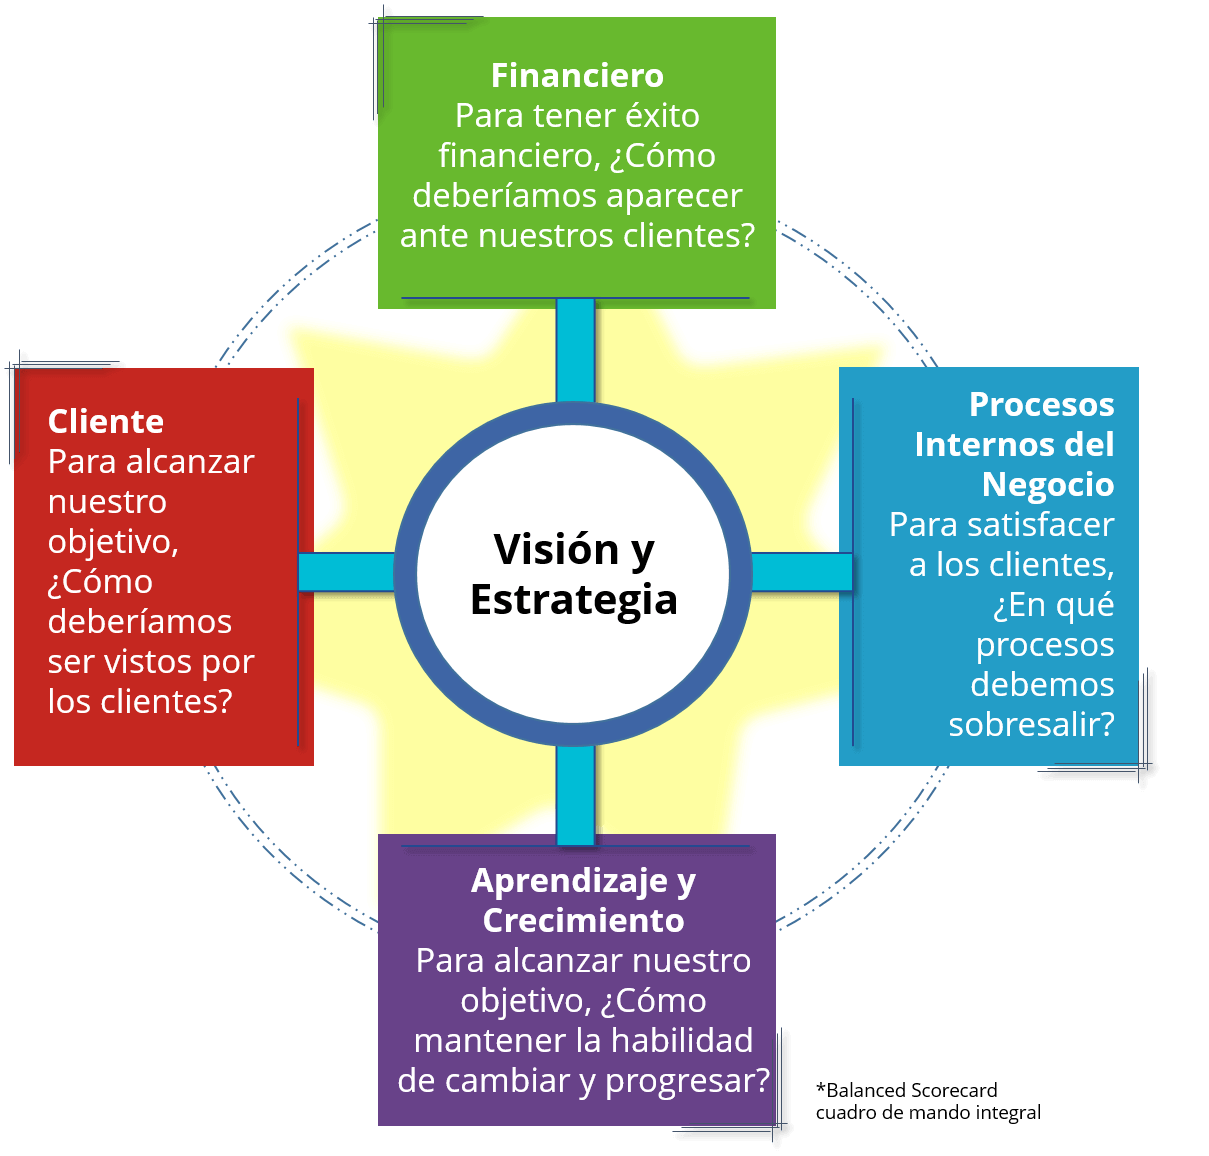
\includegraphics[width=15cm]{./Imagenes/imagen2}
\end{center}

\section{Beneficios}
\item{El Balanced Scorecard induce una serie de resultados que favorecen la administración de la compañía, pero para lograrlo es necesario implementar la metodología y la aplicación para monitorear, y analizar los indicadores obtenidos del análisis. Entre otros podemos considerar las siguientes ventajas:\\\\
-Alineación de los empleados hacia la visión de la empresa.\\
-Comunicación hacia todo el personal de los objetivos y su cumplimiento.\\
-Redefinición de la estrategia en base a resultados.\\
-Traducción de la visión y estrategias en acción.\\
-Favorece en el presente la creación de valor futuro.\\
-Integración de información de diversas áreas de negocio.\\
-Capacidad de análisis.\\
-Mejoría en los indicadores financieros.\\
-Desarrollo laboral de los promotores del proyecto.}

\begin{center}
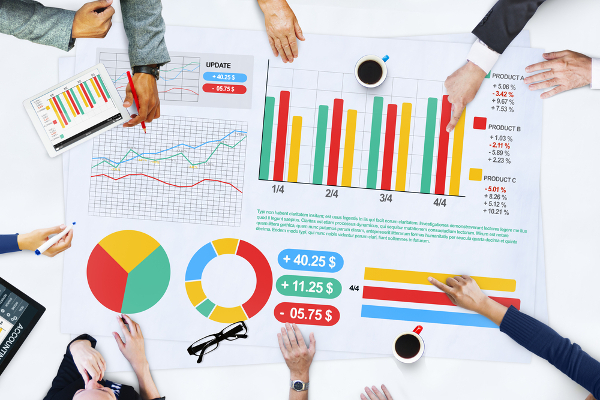
\includegraphics[width=15cm]{./Imagenes/imagen3}
\end{center}

\section{Modelo Canvas}
\item{
El modelo canvas es la herramienta para analizar y crear modelos de negocio de forma simplificada. Se visualiza de manera global en un lienzo dividido en los principales aspectos que involucran al negocio y gira entorno a la propuesta de valor que se ofrece.\\\\
El modelo canvas se utiliza para pasar de idea a proyecto y plasmar nuestra idea en un modelo empresarial. Es un modelo “vivo”, es decir, que vamos modificando según se va desarrollando, vamos validando clientes, surgen nuevas ideas… por eso se utilizan post-its para completarlo.
}

\section{Generar un modelo canvas}
\item{
Muestra de manera lógica la interconexión entre los 9 aspectos básicos de un modelo de negocio. A continuación, mostramos cómo se debe completar un modelo canvas, en qué orden y qué significa cada apartado del lienzo.\\\\
\textbf{1. Segmento de clientes}\\
Detectar las necesidades del mercado, del cliente. Nuestro foco siempre es el cliente y debemos orientar el producto a sus necesidades y deseos.\\
Para poder identificar a nuestro cliente debemos ponernos en su piel y analizar qué es lo que piensa, siente, ve, escucha, cuáles son sus problemas y los beneficios que le puede aportar nuestro producto/servicio.\\\\
Debemos dar respuesta a:\\
¿Para quién estamos creando valor?\\
¿Quiénes son nuestros clientes más importantes?
\\\\\textbf{2. Propuesta de valor}\\
Es la pieza clave de todo el modelo de negocio. La propuesta de valor o ventaja competitiva es el motivo por el que el cliente nos va a comprar a nosotros y no a otro. Aquí se incluye lo que hace diferente e innovador a nuestro producto/servicio.\\
Se puede innovar en diferentes aspectos como en el modelo de ingresos, alianzas empresariales, procesos productivos, entrega del producto/servicio, marca…\\\\
Debemos dar respuesta a:\\
¿Qué valor estamos entregando a nuestros clientes?\\
¿Qué problema resolvemos?\\
¿Cuál es la necesidad que satisfacemos?\\
¿Qué tipo de producto ofrecemos?\\\\
\textbf{3. Canales}\\
Una vez definidos nuestros clientes y la propuesta de valor que les ofrecemos, tenemos que llegar a ellos. Si no nos conocen, no nos van a comprar. Aquí vamos a definir los canales de distribución del producto o servicio.\\\\
Debemos dar respuesta a:\\
¿Con qué canales podemos llegar a nuestros clientes?\\
¿Qué canales funcionan mejor?\\
¿Cuáles de estos canales son los más rentables?\\\\
\textbf{4. Relación con los clientes}\\
Debemos comunicarnos correctamente con nuestros clientes y estar pendiente de ellos. Ellos son nuestro eje central, por lo que saber definir la relación que vamos a tener con cada segmento de clientes, es fundamental para el éxito de un negocio.\\\\
Debemos dar respuesta a:\\
¿Cuál es la relación que tenemos con cada uno de nuestros segmentos de clientes?\\
¿Qué tipo de relación esperan?\\
¿Qué coste tiene?\\\\
\textbf{5. Flujo de ingresos}\\
Para que un negocio sea rentable y podamos sobrevivir en el mercado, tenemos que pensar ¿Cómo monetizarlo? Es decir ¿De dónde vamos a obtener la facturación?\\\\
Debemos dar respuesta a:\\
¿Cuál es nuestra principal línea de ingresos? \\
¿Cómo pagarán nuestros clientes?\\
¿Por qué están dispuestos a pagar nuestros clientes?\\\\
\textbf{6. Recursos clave}
Conocer con qué recursos contamos y con los que debemos contar para llevar a cabo la actividad de nuestro negocio, es clave a la hora de establecer el plan de negocios. Debemos de ser cautos y prudentes a la hora de definir estos recursos. Siempre debemos pensar en la forma de optimizarlos, es decir, intentar conseguir la máxima productividad posible al mínimo coste.\\\\
Debemos dar respuesta a:\\
¿Qué recursos esenciales requiere nuestra propuesta de valor?\\\\
\textbf{7. Actividades clave}\\
Para llevar a cabo la propuesta de valor que queremos ofrecer a nuestros clientes, son necesarias ciertas actividades para preparar el producto antes de que llegue al mercado. Es decir, aquí pensamos en el core de nuestro negocio, lo que haremos en nuestro día a día.\\\\
Debemos dar respuesta a:\\
¿Qué actividad básica requiere nuestra propuesta de valor?\\
¿Cuáles son nuestros canales?\\
¿Cuáles son nuestras fuentes de ingresos?\\\\
\textbf{8. Aliados clave}\\
Para llevar a cabo un negocio, es imprescindible tener aliados. Estos aliados pueden ser;\\\\
Una serie de socios/colaboradores: una buena red de partners nos pueden ayudar a llegar más rápido al cliente, a ir avalados por su reputación y experiencia.\\
Los proveedores: aquellos que nos proporcionan los recursos clave para poder ofrecer los servicios/producto final.\\\\
Debemos dar respuesta a:\\
¿Quiénes son nuestros socios clave en el mercado?\\
¿Quiénes son nuestros proveedores?\\
\textbf{9. Estructura de costes}\\
Obviamente, toda esta infraestructura tiene unos costes que debemos pagar y optimizar. Debemos definir cuáles son nuestras prioridades y los gastos fundamentales en el negocio de aquellos que no lo son.\\
Tener bien clara esta estructura nos ayudará a no desviarnos de los presupuestos y que el negocio fracase por problemas de financiación.\\\\
Debemos dar respuesta a:\\\\
¿Cuáles son los costes más importantes dentro de nuestro modelo de negocio?\\
¿Qué recursos clave son los más costosos?\\
¿Qué actividades clave son las más costosas?\\
}
\begin{center}
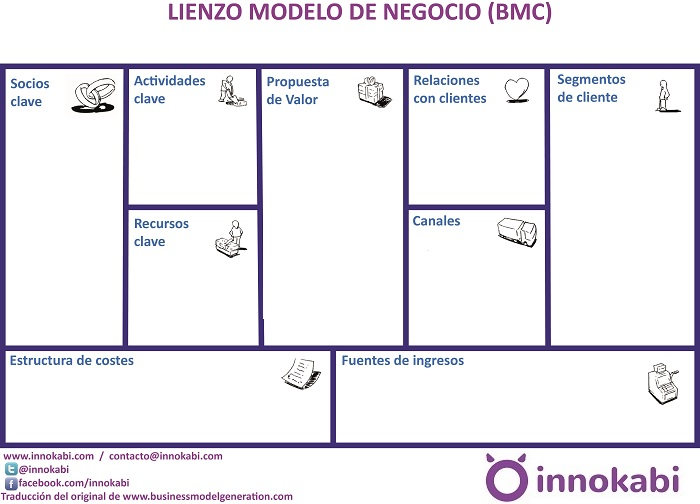
\includegraphics[width=15cm]{./Imagenes/imagen4}
\end{center}

% Bibliografía.
%-----------------------------------------------------------------
\begin{thebibliography}{99}
https://www.isotools.org/2015/02/23/que-es-el-balanced-scorecard-conoce-su-funcionamiento-y-ventajas/\\
https://economipedia.com/definiciones/modelo-canvas.html\\
http://www.infoviews.com.mx/Bitam/ScoreCard/]\\
https://innokabi.com/canvas-de-modelo-de-negocio/\\

\bibitem{Cd94} Autor, \emph{Título}, Revista/Editor, (año)

\end{thebibliography}

\end{document}
